\documentclass[a4paper,titlepage]{article}
\usepackage[czech]{babel}
\usepackage{hyperref}
\usepackage{graphicx}
\usepackage[section]{placeins}

\title{Dokumentace pro semestrální práci \protect\\ ``Booleovský model``
v rámci předmětu \protect\\``Vyhledávání na webu a v multimediálních databázích`` (BI-VWM)}

\author{Dmytro Osaulenko}

\date{\selectlanguage{czech}\today}

\begin{document}

\maketitle

\section*{Popis projektu}

Cílem projektu bylo vytvořit implementaci teoretického (booleovského) modelu
domény získávání informací (``information retrieval``), jehož hlavní myšlenkou je vyhledávání
specifických slov (termů) ve statické kolekci textů (většinou předem zpracovaných pro usnadnění
a zrychlení vyhledávání) pomocí spojek výrokové logiky jako jsou \emph{AND}, \emph{OR}, \emph{NOT}.
Uživatel by na takový vstup dostal jako výstup množinu dokumentů, pro které uvedený logický výraz
platí (případně by nedostal, pokud nějaký z termů by v kolekci nebyl přítomen, nebo by výraz z hlediska
výrokové logiky nebyl platný).

\section*{Způsob řešení}

První fází řešení je nalezení vhodné (podle velikosti a obsahu) kolekce textů (případně kolekcí textů).
Následuje předzpracování (``preprocessing``) pro optimalizaci vyhledávání a ukládání zpracovaných dat.
Jedná se hlavně o techniky NLP (``Natural language preprocessing`` nebo česky ``Zpracování přirozeného jazyka``)
jako tokenizace (``tokenization``), tj. extrakce jednotlivých slov (termů) z textu (bez interpunkce atd.),
a stematizace (``stemmming``), tj. nalezení kmene slova, nebo sofistikovanější (ale i dražší/náročnější)
operace - lemmatizace (``lemmatization``), tj. vyhledání základního tvaru slova.
\\~\\
Z mnoha variant ukládání a pak i následujícího dotazování mnou bylo zvoleno ukládat data do
\emph{hašovacích tabulek} (jinými slovy abstraktního datového typu (ADT) \emph{hašovací mapa}
(\emph{hash map}) neboli \emph{slovník} (\emph{dictionary})) anebo ještě přesněji - NoSQL databáze,
co poskytuje takovou možnost. Tak by pro každou statickou kolekci textů existovaly 2 mapy
(pro optimalizaci místa): jedna mapa by reprezentovala dokumenty v kolekci (\emph{klíč} - unikátní
identifikátor dokumentu, \emph{hodnota} - název dokumentu), druhá by reprezentovala prezenci
termů v dokumentech (\emph{klíč} - jednotlivý (stematizovaný) term, \emph{hodnota} - množina
identifikátorů dokumentů pro které platí, že term je přítomen v dokumentu).
\\~\\
Po zadání uživatelem dotazu by se ten vyhodnotil knihovnou třetí strany pro výrokovou logiku
a byl převeden na problém typu SAT (``satisfiability problem``, česky ``problém splnitelnosti``).
SAT solver knihovny by dotaz zpracoval a nabídl všechny možné varianty (pokud jsou) jak výraz
splnit a podle toho by se logická část implementace dotazovala databáze s hash mapami, sestavila by
výsledek a vrátila ho uživatelovi.

\section*{Implementace}

Z různých možností a variant pro uživatelské rozhraní jsem se rozhodl pro jednoduchou webovou stránku
(z mého pohledu nejpohodlnější a nejpřívětivější pro uživatele možnost).
Uživatelovi stačí vědět (a zadat v prohlížeči) webovou adresu aplikace a hned ji může používat
na jakémkoli svém chytrém zařízení.
\\~\\
Jako architekturu aplikace jsem zvolil klient-server. Frontendová část (klient) je implementovaná
pomocí populárního Javascript-frameworku \emph{Vue.js} a frontend knihovny CSS-stylů Bootstrap 4.
Klient řeší takové úkoly, jak je příjem dotazu od uživatele (specifikovaná kolekce textů
a booleovský výraz termů), komunikace se serverem (odesílání uživatelova požadavku a příjem odpovědi
serveru), zobrazení výsledků uživateli. Knihovna \emph{Bootstrap 4} řeší mimo jiné \emph{responsive design},
takže aplikaci se dá používat i z chytrého telefonu.
\\~\\
Backendová část (server) je implementována pomocí jazyka \emph{Python} a využívá
takové knihovny třetích stran jako:

\begin{itemize}
  \item NLTK - implementace stematizace PorterStemmer;
  \item PyEDA - parsování a validace booleovského výrazu, SAT solver;
  \item aiobotocore - asynchronní verze knihovny \emph{botocore} pro komunikaci
          se službami Amazon Web Services (AWS) (NoSQL databáze - AWS DynamoDB,
          uložiště souborů - AWS S3, výpočtová serverless jednotka - AWS Lambda).
\end{itemize}

Zpočátku bylo potřeba najít texty a zpracovat je. Rozhodl jsem se, že jednodušší variantou jak pro mě,
tak i pro uživatele budou texty v anglickém jazyce. Potom jsem chtěl nemít pouze jedinou kolekci textů,
ale alespoň několik a to z různých oborů a různé velikosti, a to jak pro zajímavost dotazu/výsledků,
tak i pro účely vývoje a ladění. Moc velká kolekce textů by se jednak dlouho zpracovávala a potom by se
v ní hledalo pomaleji, než v menší, a u menší kolekce by nastal problém řídkých a nezajímavých výsledků.
\\~\\
Zvolil jsem 3 kolekce různé velikosti a stylu: menší dump z anglické Wikipedie (největší kolekce,
cca 15 tisíc článků, cca 250 MB), 100 knih klasické světové literatury (beletrie), taky anglicky,
přesněji tedy 100 knih ze stránky ``Top 100 EBooks yesterday`` projektu Gutenberg (cca 60 MB) a nejmenší
kolekci je bibliografie moderního amerického spisovatele Chucka Palahniuka (cca 20 knih, cca 6 MB).
Všechny soubory byly ve formátu .txt, nic méně skript, co zpracovává texty používá knihovnu
\emph{textract} co umí raw text vytáhnout ze souborů různých
formátů (např .pdf, .docx, .epub atd.), takže tato implementace tuto možnost také podporuje.
\\~\\
Během vývoje a ladění jsem používal lokální (vývojářský) server na backendu (knihovna \emph{aiohttp}),
frontend byl hostovan také lokálním serverem pro frontend. První experimenty se prováděly nad soubory
formátu JSON a potom i v NoSQL databází běžící na lokálním počítači (např. MongoDB).
Nic méně pro účel zveřejnění a fungování webové aplikace bylo potřeba ji nasadit (``to deploy``) do
produkčního prostředí. Rozhodl jsem se používat služby Amazon Web Services (dále AWS), a to AWS Lambda
pro backend, AWS DynamoDB jako NoSQL databázi, AWS S3 pro hosting statického webu. Navíc jsem
implementoval možnost po obdržení výsledků jednotlivé dokumenty si prohlédnout, případně
stáhnout, dokumenty příslušné kolekce jsou také uloženy na AWS S3.
Aby frontend (z S3 bucketu) mohl komunikovat s ``lambdou`` bylo nastaveno REST API pomocí AWS ApiGateway.
Celkové schéma aplikace bude znázorněno trochu níže na obrázku.
\\~\\
Bohužel ve zdrojových kódech (kvůli časovým možnostem) není verze pro úplně lokální běh aplikace,
bez využití jakýchkoli ``cloud`` služeb (až na lokální server místo AWS Lambda), hodně se to spoléhá
na DynamoDB a S3.
\clearpage

\begin{figure}[t]
\centering
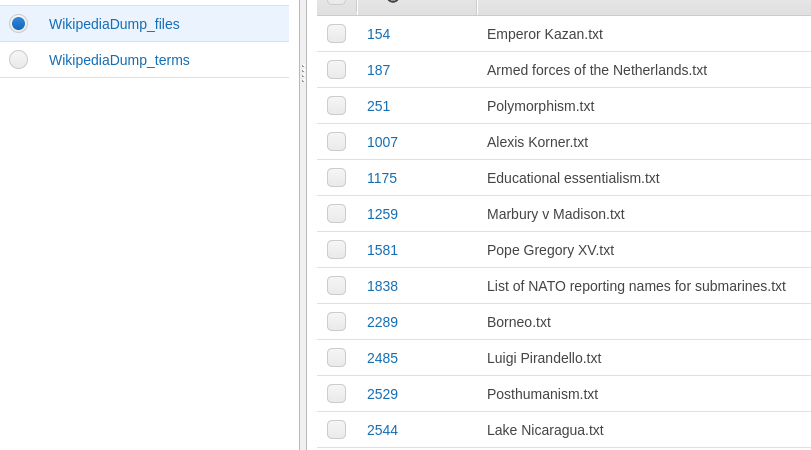
\includegraphics[scale=0.5]{DynamoDB_table_files_structure.png}
\caption{
DynamoDB, kolekce WikipediaDump,
mapa identifikátor dokumentu (klíč): název dokumentů (hodnota)
}
\end{figure}

\begin{figure}[h]
\centering
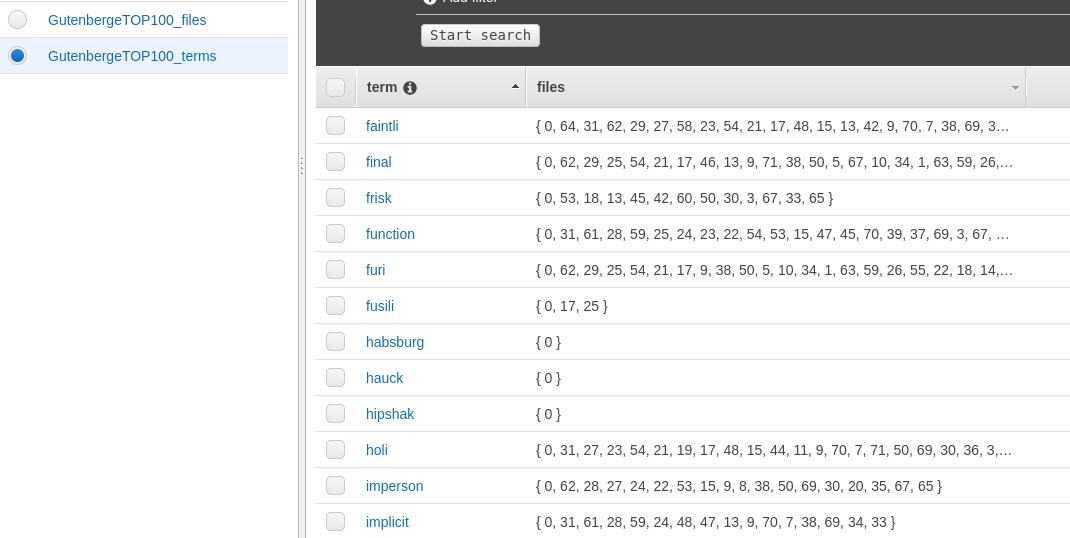
\includegraphics[scale=0.4]{DynamoDB_table_terms_structure.png}
\caption{
DynamoDB, kolekce GutenbergTOP100, mapa term (klíč):
množina identifikátorů dokumentů (hodnota)
}
\end{figure}

\begin{figure}[h]
\centering
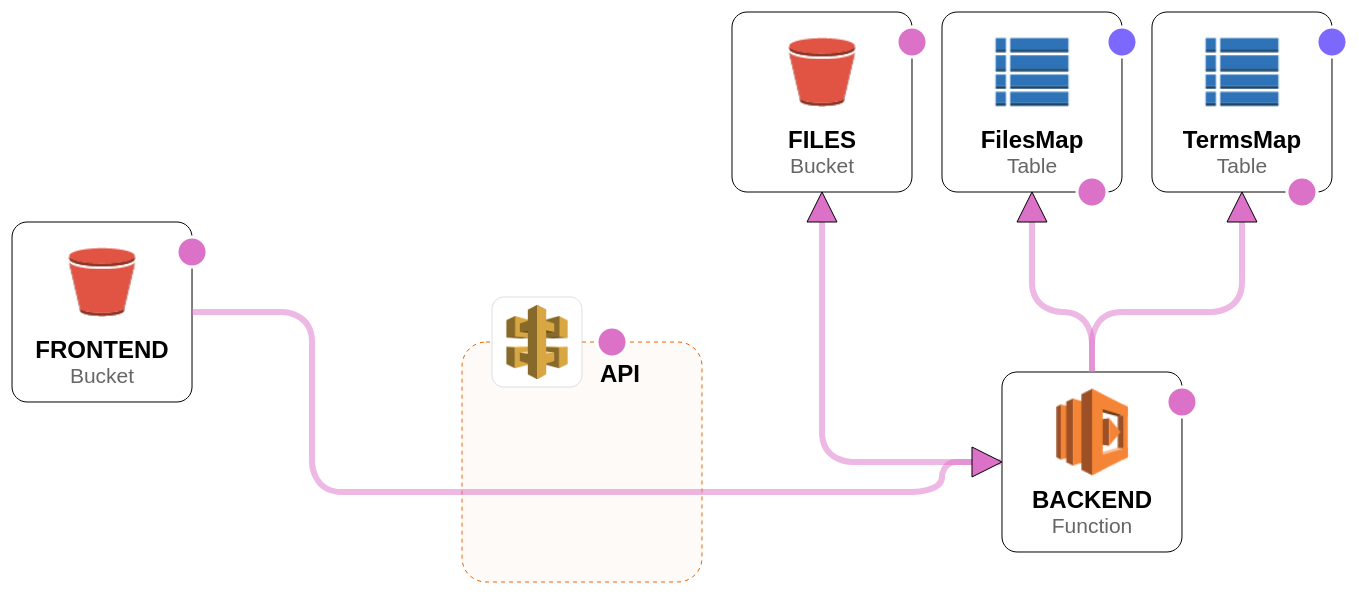
\includegraphics[scale=0.3]{architecture_scheme.png}
\caption{
Schéma architektury finální nasazené aplikace:
frontend (AWS S3 bucket) volá backend AWS Lambda přes AWS ApiGateway.
Lambda-backend dělá dotaz na tabulky v DynamoDB a vrací spočítaný výsledek na frontend.
Pokud uživatel požádá o zpřístupnění jednotlivého dokumentu, frontend odešle takový
požadavek backendu a backend vrátí link (expirující za 5 minut) na požadovaný soubor.
}
\end{figure}

\section*{Příklad výstupu}

\begin{figure}[h]
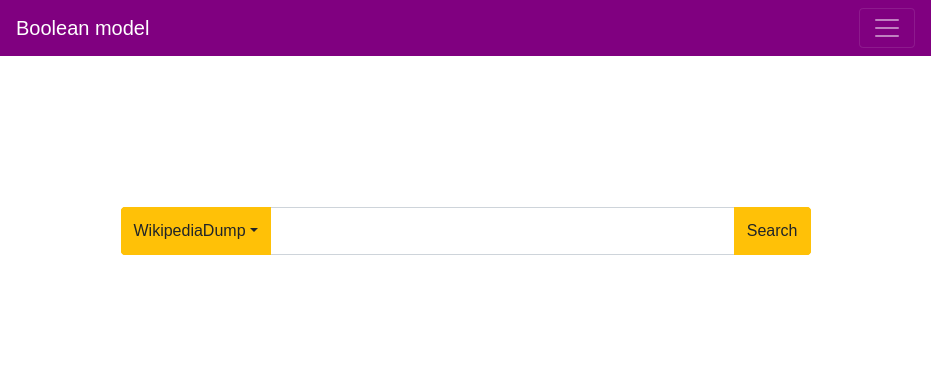
\includegraphics[scale=0.4]{Frontend_search_page.png}
\caption{Hlavní stránka vyhledávání. Do příslušného pole uživatel zadává hledaný výraz.
V levém dropdownu lze zvolit kolekci textů, nad jakou bude dotaz proveden.
}
\end{figure}

\begin{figure}[h]
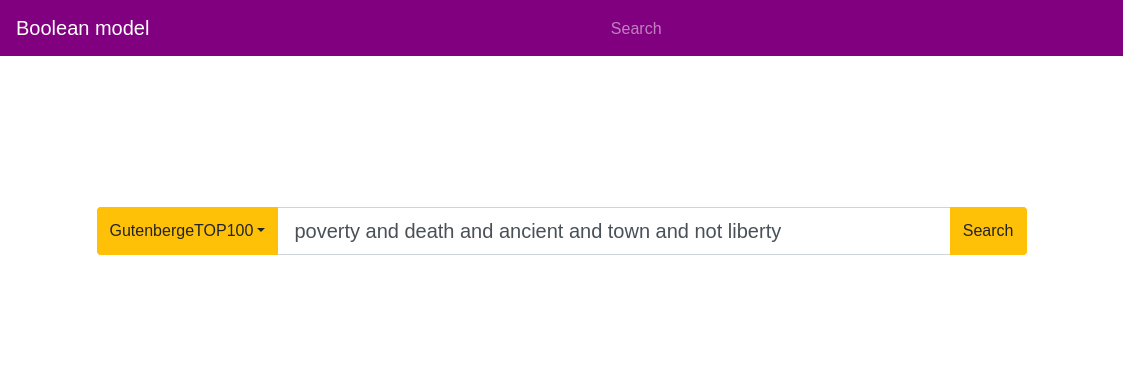
\includegraphics[scale=0.35]{Frontend_search_page_with_query.png}
\caption{Zadání výrazu. Po kliknutí na \emph{Search} se dotaz odešle
logické části, ta jeho zhodnotí a vrátí výsledky.}
\end{figure}

\begin{figure}[h]
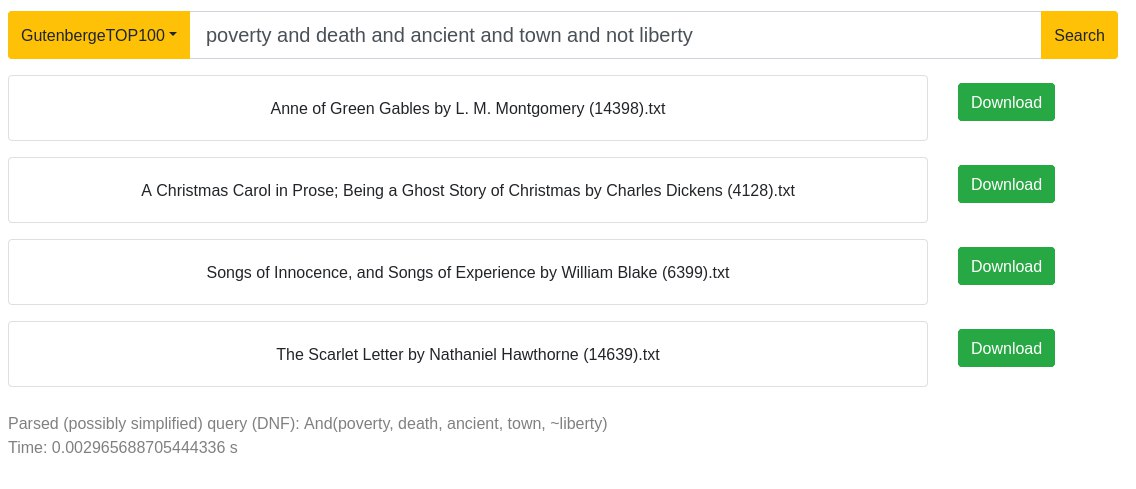
\includegraphics[scale=0.35]{Frontend_query_results.jpg}
\caption{Výsledky, pro které dotaz (logický výraz) platí.
Při kliknutí na \emph{Download} může si uživatel dokument prohlédnout.}
\end{figure}


\section*{Experimentální sekce}

U malých dotazů (např. pouze ``dog``) čas po stisknutí \emph{Search} je o hodně větší,
než u dotazů s více termy. Pokud nějaký term nebude v mapě existovat,
ale bude například součástí výrazu s velkým množstvím AND spojek, vyhodnocení
výsledků bude o hodně rychlejší. Nic méně u malých kolekcí textů ten rozdíl zas tak velký ale nebude.
\\~\\
Příklady:

\begin{table}[h!]
\centering
\begin{tabular}{||c c c||} 
 \hline
 Dotaz & Kolekce & Čas [s]\\ [0.5ex] 
 \hline\hline
 dog & WikipediaDump & 19.88 \\ 
 dog and cat & WikipediaDump & 4.76 \\
 foo or foobar & WikipediaDump & 0.98 \\
 not (dog or cat) & WikipediaDump & 0.34 \\
 programming and computes and python and javascript & WikipediaDump & 1.00 \\
 \hline
\end{tabular}
\caption{Dotazy, kolekce textů, čas na vyhodnocení dotazu}
\end{table}

Výše uvedené časy jsou použity z footeru stránky po vyhodnocení a obdržení výsledků.
Časem vyhodnocení je míněn rozdíl času od zahájení vyhodnocení výrazu po vrácení výsledků.

\section*{Diskuze}

Hlavním nedostatkem booleovského modelu je absence ceny termů. Tento nedostatek je vyřešen
v tzv. \emph{Rozšířeném booleovském modelu} (``Extended boolean model``).
\\~\\
Jako rozšíření zadání jsem chtěl udělat možnost mít dynamickou kolekci textů (s přidáváním nových
dokumentů nebo mazáním starých) nebo i vytvářet nové kolekce, nic méně tato rozšíření by potřebovala
další čas pro vývoj.

\section*{Závěr}
Jsem rád, že jsem se v předmětu \emph{BI-VWM} blíž seznámil s doménou \emph{information retrieval},
s jedním z její teoretických modelů - \emph{booleovským} a měl jsem zkušenost ho implementovat.

Bavilo mě to a ohromnou část času, co jsem u toho ztrávil, jsem spíše vymýšlel rozmanitá
rozšíření zadání a implementace, než samotný algoritmus.

Nakonec jsem se k zadání vrátil a to dodělal, i když ne tak, jak jsem to začátku viděl a chtěl,
ale jsem s finální implementací spokojen.

Nic méně díky této úloze mám inspiraci dělat ve volném čase projekty podobného typu.
\end{document}
